% !TEX root = ../main.tex

\section{Preliminaries}

\subsection{How \textit{multiple withdrawal attack} works}

\noindent According to the ERC20 API definition:

\begin{compactlist}
\item The \texttt{approve} function allows spender to withdraw up to allowed tokens from token pool of the approver. If this function is called again, it overwrites the current allowance with the new input value.
\item The \texttt{transferFrom} function allows the spender (\eg user, wallet or other smart contracts) to transfer tokens on behalf of the approver. It updates balance of transaction parties accordingly.
\end{compactlist}
An adversary can exploit the gap between execution of \texttt{approve} and \texttt{transferFrom} functions since the \texttt{approve} method overrides current spender allowance regardless of whether the spender already transferred any tokens or not. This functionality of the \texttt{approve} method is defined by the standard and cannot be changed. Furthermore, transferred tokens are not trackable and only \texttt{Transfer} events are logged, which is not sufficient in case of transferring tokens to a third party (i.e., \texttt{Transfer} event will not be related to the spender). To make it clear, the following attack scenario can be applied:

\begin{compactlistn}
	\item Alice allows Bob to transfer N tokens on her behalf by executing \texttt{approve(\_Bob, N)}.
	\item Later, Alice decides to change Bob's approval from N to M by calling \texttt{approve(\_Bob, M)}.
	\item Bob notices Alice's second transaction after it is broadcast to the Ethereum network but before it is added to a block.
	\item Bob using the asymmetric insertion method~\cite{eskandari2019sok} and front-runs the original transaction to run  \texttt{transferFrom(\_Alice, \_Bob, N)} first. If a miner is incentivized to add this transaction before Alice's, it will transfer N Alice's tokens to Bob before changing Bob's approval.
	\item Alice's transaction will be executed after Bob's.
	\item Bob can call \texttt{transferFrom} method again and transfers M additional tokens by executing \texttt{transferFrom(\_Alice, \_Bob, M)}.
\end{compactlistn}
In summary, in attempting to change Bob's allowance from N to M, Alice makes it possible for Bob to transfer N+M of her tokens. We operate on the assumption that a secure implementation would prevent Bob from withdrawing Alice's tokens multiple times when the allowance changes from N to M (see Figure~\ref{fig:mwa}). If Bob could withdraw N tokens after Alice initial approval, this would be considered as legitimate transfer, since Alice has already approved it. In other words, it would be the responsibility of Alice to make sure tokens have not been transferred before modifying her approval for Bob.
\begin{figure}[ht]
	\centering
	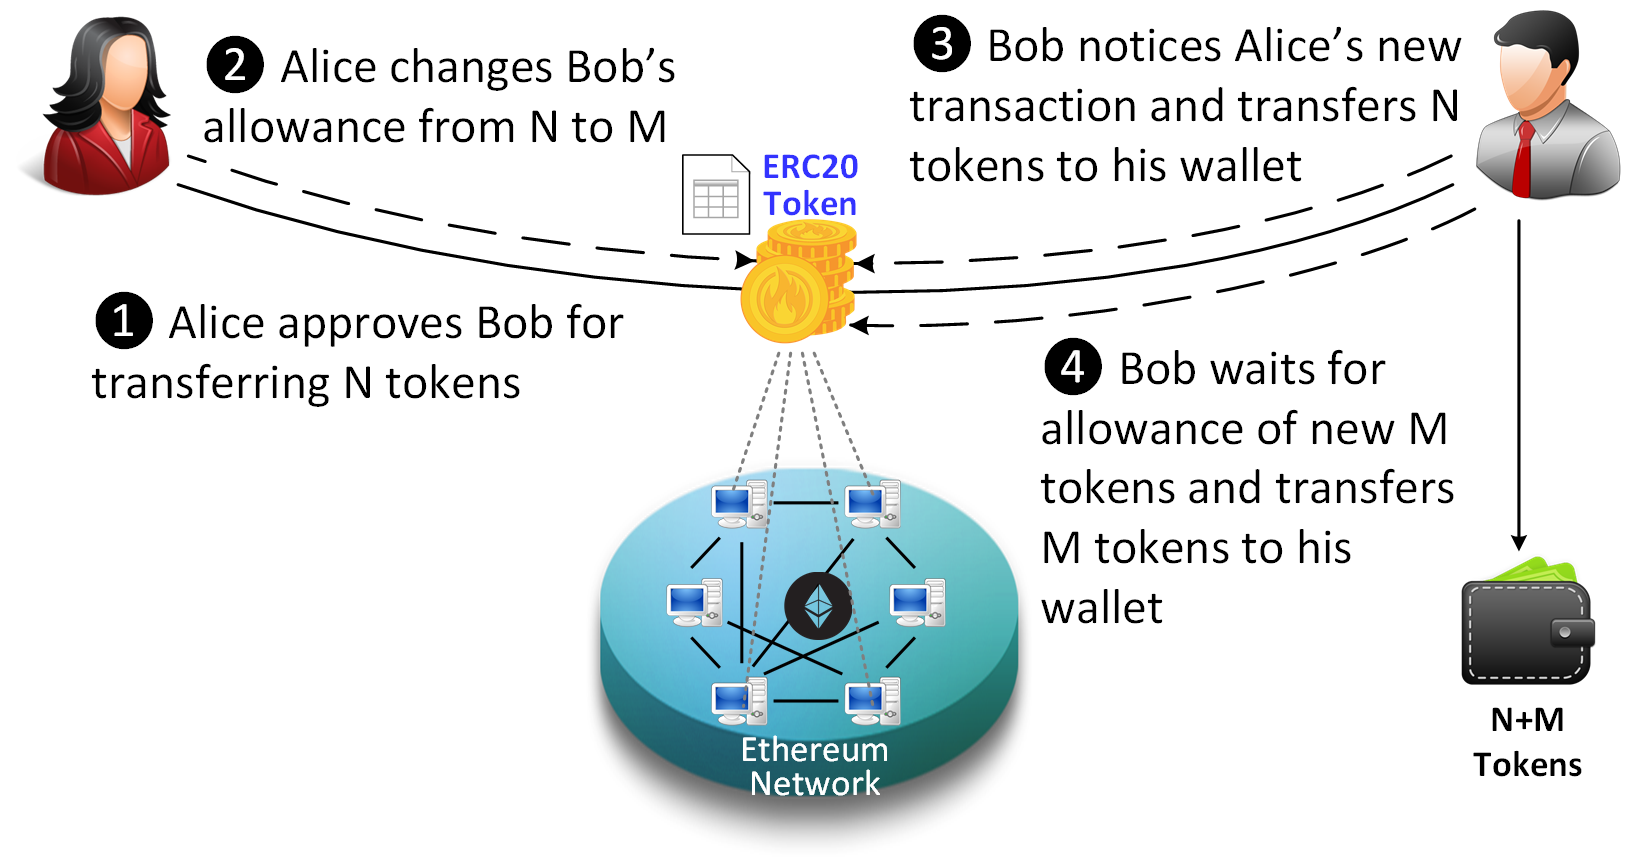
\includegraphics[width=1.0\linewidth]{figures/multiple_withdrawal_02.png}
	\caption{Possible multiple withdrawal attack in ERC20 tokens when Alice changes Bob's allowance from N to M. By front-running, Bob is able to move N+M tokens from token pool of Alice.\label{fig:mwa}}
\end{figure}

\subsection{Importance of mitigation}
To effect this attack, there is a need for executing mining code and tracking transactions before being added to the block. It is therefore not easy to execute and requires initial preparation. The reason for mitigating it can be one of the followings:
\begin{compactlist}
	\item As the Token becomes valuable, the possibility of this attack is likely. An ERC20 token can represent different type of financial assets. From company shares to fiat currency. This might be an incentive to launch the attack.
	\item ERC20 tokens are widely used in distributed applications and has to be secure in order to secure the entire system.
	\item Ethereum tokens are regularly under audit and this vulnerability can be against best practices and increasing potential attack surface.
\end{compactlist}

\subsection{General prevention techniques}

\noindent In general, there would be off-chain and on-chain transaction to consider when proposing solutions. For this paper, off-chain transactions are out of scope. Therefore, concentration will be on on-chain prevention techniques:
\begin{enumerate}
	\item \textbf{Prevention by token owner}: Considering owner responsibility to mitigate the attack in UI (\eg Web3.js) instead of contract (\ie Solidity/Vyper).
	\item \textbf{Prevention by token author}: Smart contract author(s) have to mitigate the attack by securing either \texttt{approve} or \texttt{transferFrom} methods.
\end{enumerate}

\subsubsection*{Prevention by token owner} This approach is recommended by ERC20 authors \cite{Ref08} and advises token holder to change spender allowance from N to zero before zero to M (instead of directly from N to M). This will not prevent the attack because changing of allowance from N to zero by the owner is indistinguishable from transferred tokens by the attacker. In other words, after execution of \texttt{approve} function, token holder sees allowance=0, but cannot distinguish whether it was because of execution of \texttt{approve} method or has been set to zero in \texttt{trnasferFrom} function due to token transfer. Although it would be possible to track transferred tokens through \texttt{Transfer} events, but it would miss some information in case the transfer happens to a third-party. For example, if Alice allows Bob to transfer N tokens, Bob can transfers N tokens to anyone not just to himself. He might call \texttt{transferFrom(\_Alice, \_Carol, N)} to transfer the N tokens to Carol. In this case, \texttt{Transfer}\footnote{\texttt{Transfer} event is defined as \texttt{Transfer(address \_from, address \_to, uint256 \_tokens)}. It does not log \texttt{msg.sender} who called \texttt{transferFrom} function. Therefore, Bob can easily call \texttt{transferFrom} by specifying address of someone else (\texttt{\_from}=Alice's address, \texttt{\_to}=Carol's address).} event creates a log showing Carol moved N tokens from Alice with no indication that it was instigated by Bob. As discussed later in~\ref{sec:MiniMeToken}, this approach can not prevent the attack since it is not distinguishable which transaction (\ie owner or spender transaction) has set the allowance to zero. Consequently, Alice cannot decide whether to change Bob's allowance to M or not. Changing his allowance to M might allow Bob to transfer more M tokens (N+M in total) and not changing it will prevent any legitimate allowance change.

%SHAYAN: maybe we should separate (or mention) off-chain detections (e.g events) and on-chain detection. in order to prevent such attacks I believe on-chain solutions are required. however I have to go through all the proposals to have a more complete opinion about this.
% Jeremy: Agreed. We declare off-chain out of scope for the paper
	
\subsubsection*{Prevention by \texttt{approve} method} Securing \texttt{approve} method could be a solution and prevent the attack. By using compare and set (CAS) pattern \cite{Ref06}, \texttt{approve} method can change spender allowance from N to M atomically (\ie comparing new allowance with transferred token and set it accordingly). Comparison part of CAS requires knowledge of previously transferred tokens that will reveal any token transfer in case of front-running. Although this is promising approach,  setting new allowance in \texttt{approve} method must satisfy ERC20 constraint that dictates "If this function is called again it overwrites the current allowance with \texttt{\_value}" \cite{Ref08}. This does not allow any adjustments in allowance while it is a prerequisite for securing \texttt{approve} method. 
%SHAYAN: REZA I'm not sure what this example is.
For example, considering front-running by Bob when Alice changes his allowance form 100 to 110, the \texttt{approve} method can reveal 100 transferred tokens by Bob and has to set Bob allowance to 10 (110-100=10). However, based on ERC20 constraints, it must not adjust the allowance and has to set it literally to 110. Consequently, this allows Bob to transfer 100+110=210 tokens in total. We implemented this approach in~\ref{sec:proposal1} and concluded that securing \texttt{approve} method cannot prevent the attack while adhering constraints of the ERC20 standard.
	
\subsubsection*{Prevention by \texttt{transferFrom} method} Based on ERC20 specifications, "approve functions allows \texttt{\_spender} to withdraw from your account multiple times, up to the \texttt{\_value}". Therefore, spender must not be able to transfer more than allowed tokens. That being said, \texttt{transferFrom} method can prevent transferring of new tokens in case of already transferred tokens up to allowed amount. By comparing transferred tokens in \texttt{transferFrom} method, spender will be restricted to move solely the remaining tokens of his allowance. In case of trying to transfer more tokens than allowed, the transaction fails. For example, Alice's new transaction for increasing Bob allowance from 100 to 110, sets Bob allowance to 110 (\texttt{approve} method sets allowance regardless of transferred tokens). However, \texttt{transferFrom} method prevent the attack by not allowing Bob to transfer more than 10 tokens if he had already transferred 100 tokens. We implemented this approach in~\ref{sec:proposal2} and it mitigates the attack effectively.

\subsection{Properties of acceptable solutions}
An important criterion for a solution is to adhere the specifications of ERC20 standard. Conforming with the standard ensures that new tokens are backward-compatible with already deployed smart contracts or web applications. We summarized ERC20 constraints \cite{Ref08} that must be satisfied by any sustainable solution:


%SHAYAN: REZA isn't the second item the same as the first item? 
\begin{enumerate}
	\item Calling \texttt{approve} function has to overwrite current allowance with new allowance.
	\item \texttt{approve} method does not adjust allowance, it sets new value of allowance.
	\item Transferring 0 values by \texttt{transferFrom} method MUST be treated as normal transfers and fire the \texttt{Transfer} event as non-zero transactions.
	\item Spender will be allowed to withdraw from approver account multiple times, up to the allowed amount.
	\item Transferring initial allowed tokens is considered as legitimate transfer. It could happen right after approval or before changing it.
	\item Race condition MUST not happen in any case to prevent multiple withdrawal from the account.
	\item Introducing new methods violate ERC20 API and MUST be avoided for having compatible token. In other words, introducing new secure methods that are not defined in the initial ERC20 API, make them unusable with already deployed smart contracts. Therefore, smart contracts cannot use them to prevent the attack.
\end{enumerate}